%! Author = mddzi
%! Date = 02.06.2024

% Preamble
\documentclass[12pt,a4paper,twoside]{report}

% Packages
\usepackage{amsmath}
\usepackage[T1]{fontenc}
\usepackage[utf8]{inputenc}
\usepackage{lmodern}
\usepackage{textcomp}
\usepackage{lastpage}
\usepackage{geometry}
\usepackage{graphicx}
\usepackage{fancyhdr}
\usepackage[svgnames]{xcolor}
\usepackage[font={small,color=Grey},labelsep=period,width={0.8\textwidth}]{caption}
\usepackage{float}
\usepackage{multirow}
\usepackage{subcaption}
\usepackage{adjustbox}
\usepackage{longtable}
\usepackage{etoolbox}
\usepackage{hyperref}
\usepackage{pdfpages}
\usepackage{indentfirst}
\usepackage{icomma}
\usepackage{natbib}
\usepackage{microtype}
%\usepackage{lstmisc}
%\usepackage[backend=bibtex, sorting=none]{biblatex}

\geometry{margin=3.5cm}

\renewcommand{\figurename}{Rysunek}
\renewcommand{\chaptername}{Rozdział}
\renewcommand{\contentsname}{Spis treści}
\renewcommand{\bibname}{Bibliografia}

\pagestyle{fancy}

\title{\textbf{Program do tworzenia schematów układów scalonych w formie gry edukacyjnej}\\[2ex]
    \large Program for creating IC diagrams in the form of an educational game\\
}
\author{Maksymilian Dziemiańczuk}
\date{}

\fancyhf{}
\fancyhead{}
\fancyhead[RO,LE]{Maksymilian Dziemiańczuk}
\fancyhead[RO,LE]{Projekt inżynierski}
\fancyfoot{}
\fancyfoot[RO,LE]{\thepage}
\fancyfoot[RE,LO]{\footnotesize Program do tworzenia schematów układów scalonych w formie gry edukacyjnej}
\fancypagestyle{plain}{
    \renewcommand{\headrulewidth}{0pt}
    \fancyhf{}
    \fancyfoot[RO,LE]{\thepage}
    \fancyfoot[RE,LO]{\footnotesize Program do tworzenia schematów układów scalonych w formie gry edukacyjnej}
}

% Document
\begin{document}

%\maketitle
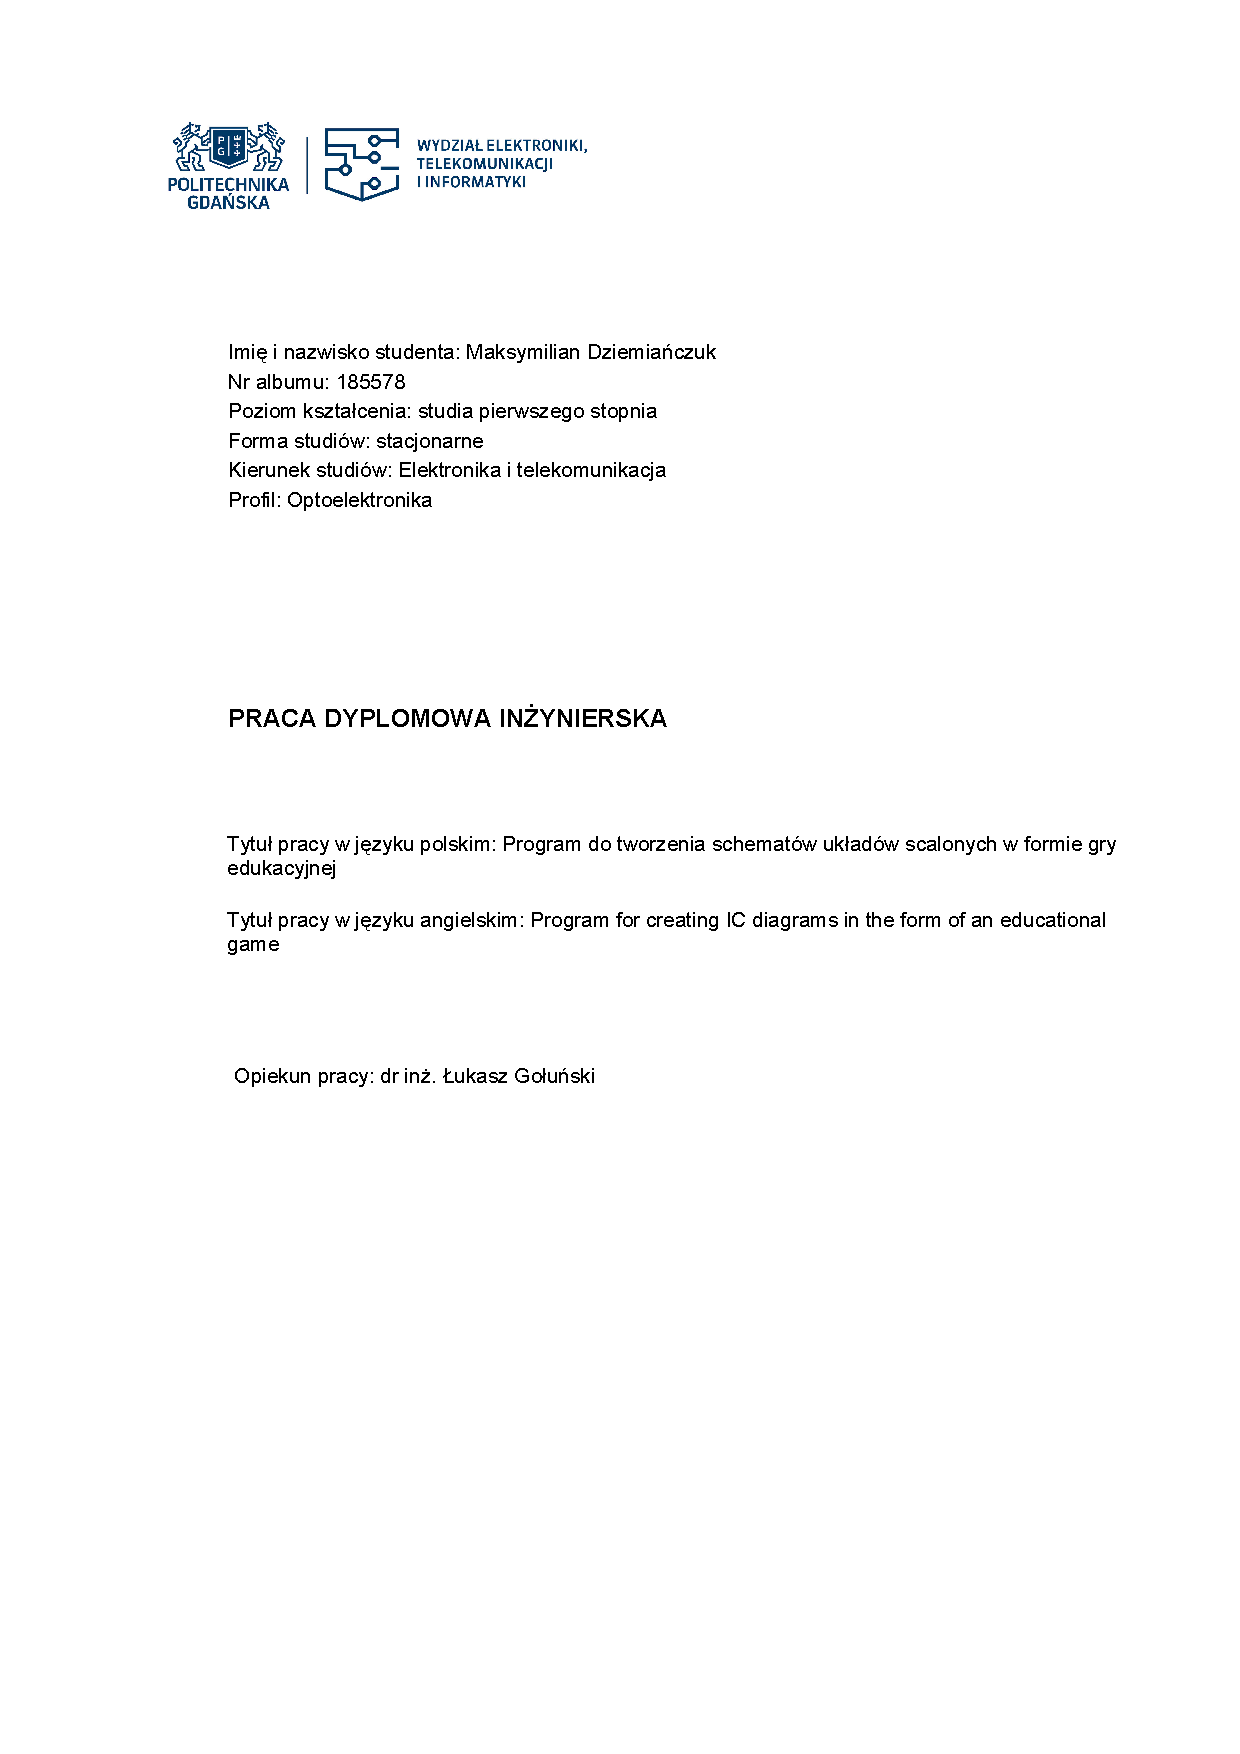
\includepdf[pages={1}]{StronaTytulowa_185578.pdf}

%pusta strona
\newpage \thispagestyle{empty} \ \newpage

\section*{Streszczenie}
\thispagestyle{plain}

Lorem ipsum dolor sit amet, consectetur adipiscing elit

\tableofcontents

\chapter{Wstęp i cel pracy}

Programy do tworzenia schematów są jednym z~kluczowych elementów
procesu wielkoskalowej integracji układów scalonych (ang. VLSI — Very Large Scale Integration)~\cite{VLSI_insemi}.
Polega to na projektowaniu podukładów o określonych funkcjach,
które następnie są łączone w~jeden, w~pełni działający układ scalony.
Taki proces upraszcza projektowanie oraz produkcję układów scalonych, ponieważ prace można podzielić na mniejsze,
mniej skomplikowane części.
Dodatkowo wiele podukładów może być wykorzystywanych w~różnych projektach,
co~znacznie zwiększa efektywność pracy i~obniża jej koszty.
W~efekcie,
programy wspierające projektowanie schematów są nieodzownym narzędziem przy tworzeniu układów scalonych.
%w~ten sposób upraszczany jest proces projektowania oraz produkcji układów scalonych,
%gdyż pracę można podzielić na mniejsze części,
%a~dodatkowo cześć podukładów może być używana w~wielu różnych projektach.
Przykładem takiego programu jest open-source'owy (o publicznym kodzie źródłowym),
Magic VLSI stworzony przez Johna Ousterhouta w~1980 roku,
napisany w~języku C na platformę Linux~\cite{MAGIC_article}.
Charakteryzuje go prosta szata graficzna oraz szeroki zakres działania,
lecz jego obsługa bywa często nieintuicyjna oraz nieprzyjazna dla początkujących użytkowników.
Kolejnym powszechnie dostępnym programem jest Microwind,
na który składa się zestaw modułów,
jednym z~nich jest edytor schematów~\cite{Microwind}.
Niestety, aby używać pełnej i~aktualnej wersji oprogramowania potrzebna jest licencja.
W~wielu innych przypadkach programy te~są~dostępne jedynie w~wersjach płatnych, kierowanych do dużych firm.
To właśnie wysoki próg wejścia
i~złożoność obsługi tego rodzaju programów stały się inspiracją do opracowania tego projektu.\\
%\indent Celem tej pracy było stworzenie
%programu edukacyjnego w~formie gry, który pomoże w~nauce tworzenia schematów układów scalonych,
%ponieważ już same gry komputerowe, nawet te~niemające wyraźnie edukacyjnego charakteru,
%mogą rozwijać umiejętności graczy dzięki stawianiu przed nimi angażujących wyzwań
%i~zachęcaniu do rozwiązywania problemów w kreatywny sposób~\cite{videogames}.\\
\indent Celem tej pracy było opracowanie programu edukacyjnego w~formie gry,
który pomoże w nauce tworzenia schematów układów scalonych.
Gry komputerowe, nawet te~niemające wyraźnie edukacyjnego charakteru,
mogą rozwijać umiejętności graczy.
Osiągają to~poprzez stawianie przed nimi angażujących wyzwań oraz zachęcanie do kreatywnego rozwiązywania problemów~\cite{videogames}.\\
\indent Jedne z~głównych programu założeń to prostota obsługi, intuicyjność oraz ergonomia,
na które mają wpływ przede wszystkim dobrze zaprojektowany interfejs graficzny użytkownika
oraz wbudowane narzędzia wspierające edycję schematu.
%Na tych założeniach opiera się cała część projektu związana z~interfejsem użytkownika.\\
Funkcje te~stanowią podstawę części projektu związaną z~interfejsem użytkownika
i~odpowiadają za poprawę użyteczności
oraz dostępność aplikacji.\\
\indent Kolejnym istotnym elementem tej pracy było przygotowanie angażującej
i~skalowalnej pętli rozgrywki,
która pozwoli na stopniowe wprowadzanie użytkownika w~proces projektowania schematów układów scalonych,
wraz z~implementacją systemów sprawdzania poprawności wykonanych zadań, wskazywania błędów i~ewentualnych podpowiedzi.
%Dzięki realizacji założeń program pomoże w~nauce podstaw bez odrzucania użytkownika
%przez zbyt skomplikowaną obsługę.\\
Dzięki realizacji założeń, projekt ten pozwoli użytkownikowi na zdobycie podstawowej wiedzy
i~umiejętności z~zakresu projektowania układów scalonych,
bez konieczności przechodzenia przez trudniejsze w~obsłudze, tradycyjne oprogramowanie.\\
\indent Zważając na wszystkie założenia oraz charakter edukacyjno-growy projektu,
do realizacji wybrano silnik Unity Engine,
bazujący na języku C\#,
powszechnie wykorzystywany w~tworzenia gier komputerowych.
%program został stworzony w~silniku Unity Engine,
%powszechnie używanym do tworzenia gier komputerowych.
%natomiast możliwość łatwego tworzenia interaktywnej aplikacji graficznej sprawdzi się w~tego typu zastosowaniach.\\
Wybór Unity podyktowany był prostotą tworzenia aplikacji graficznych oraz łatwego tworzenia interaktywnych elementów,
co~można wykorzystać nie tylko w~grach, ale również w~różnego typu narzędziach.
Dzięki Unity,
program łączy funkcje gry z~elementami edukacyjnymi,
tworząc przystępną i~atrakcyjną platformę do nauki podstaw projektowania układów scalonych.
%Został on wybrany ze względu na prostotę tworzenie aplikacji graficznych oraz łatwego tworzenia interaktywnych elementów,
%coi~można wykorzystać nie tylko w~grach, ale również w~różnego typu narzędziach.
%Aby ujednolicić schematy oraz zadania do wykonania dla użytkowników,
%projektowanie będzie odbywać się w~tylko jednej technologii\ \textendash \ CMOS AMIS ami-C5.
%Powodem wyboru tej technologii jest wcześniejsze doświadczenie w~projektowaniu schematów układów scalonych
%w~tej technologii.

\chapter{Przegląd istniejących rozwiązań}

Projektowanie topografii jest obecnie istotnym elementem procesu tworzenia współczesnej elektroniki,
wymagającym zarówno solidnej wiedzy teoretycznej, jak i umiejętności praktycznych korzystania z odpowiednich narzędzi.
Dostępne na rynku programy wspierające ten proces oferują wiele zaawansowanych funkcji,
ale ich złożoność oraz częsta potrzeba posiadania płatnej licencji ogranicza ich przystępność dla osób początkujących.\\
\indent Istniejące rozwiązania mogą wskazać jakie funkcje, zarówno podstawowe, jak i zaawansowane,
powinny zostać zaimplementowane w programie.
Analiza ich zalet, ograniczeń, jak również przystępności dla użytkowników pozwala określić,
w jaki sposób unikać problemów z intuicyjnością i ergonomią interfejsu jednocześnie wykorzystując sprawdzone mechanizmy.\\
\indent Poza programami do tworzenia schematów należy również przyjrzeć się innym profesjonalnym lub półprofesjonalnym narzędziom,
co pozwoli na zrozumienie, jak powinien być zaprojektowany schludny i intuicyjny interfejs użytkownika.

\section{Magic VLSI}

Jednym z bardziej popularnych oraz najbardziej dostępnych programów do projektowania układów scalonych
jest Magic VLSI\@.
Opracowany w 1983 roku przez Johna K. Ousterhouta i jego zespół na Uniwersytecie Kalifornijskim w Berkeley,
napisany w języku C, pierwotnie dla systemu Berkeley 4.2 będącego wariacją platformy Unix~\cite{MAGIC_article}.
Program ten posiada własną stronę internetową, na której można znaleźć dokumentację, kod źródłowy,
wskazówki dotyczące projektowania schematów, jak również pobrać program~\cite{MAGIC_site}.
Dzięki otwartemu kodowi źródłowemu oraz wysokiej funkcjonalności Magic zyskał dużą popularność
w środowiskach akademickich i naukowych, a także wśród hobbystów.
Jego główną jest brak konieczności posiadania płatnej licencji,
przy czym jednocześnie pozwala na pełne zaprojektowanie schematu układu scalonego.\\
\newpage
\indent Unikalną cechą programu Magic jest wprowadzenie techniki strukturyzacji danych
zszytych narożników \textit{corner-stitched},
która znacząco poprawia jego wydajność.
Mechanizm ten opiera się na reprezentacji układu scalonego jako zestaw warstw,
na które składa się zestaw prostokątnych komórek.
%(ang. \textit{cells}).
Każda komórka zawiera zszyte narożnikami powierzchnie (ang. \textit{corner-stitched planes}),
opisujące jej geometrię oraz podkomórki, a każda z nich składa się z wielu prostokątnych kafelków.
Taka struktura pozwala na szybkie i efektywne operacje na schemacie,
takie jak znajdywanie wszystkich kafelek w danym obszarze lub sąsiadów danej komórki,
a także przeszukiwanie połączonych regionów kafelków.
Dzięki zastosowanym mechanizmom możliwe jest także wykonywanie operacji na dużych obszarach
i szybką aktualizację danych.

\begin{figure}[h]
    \centering
    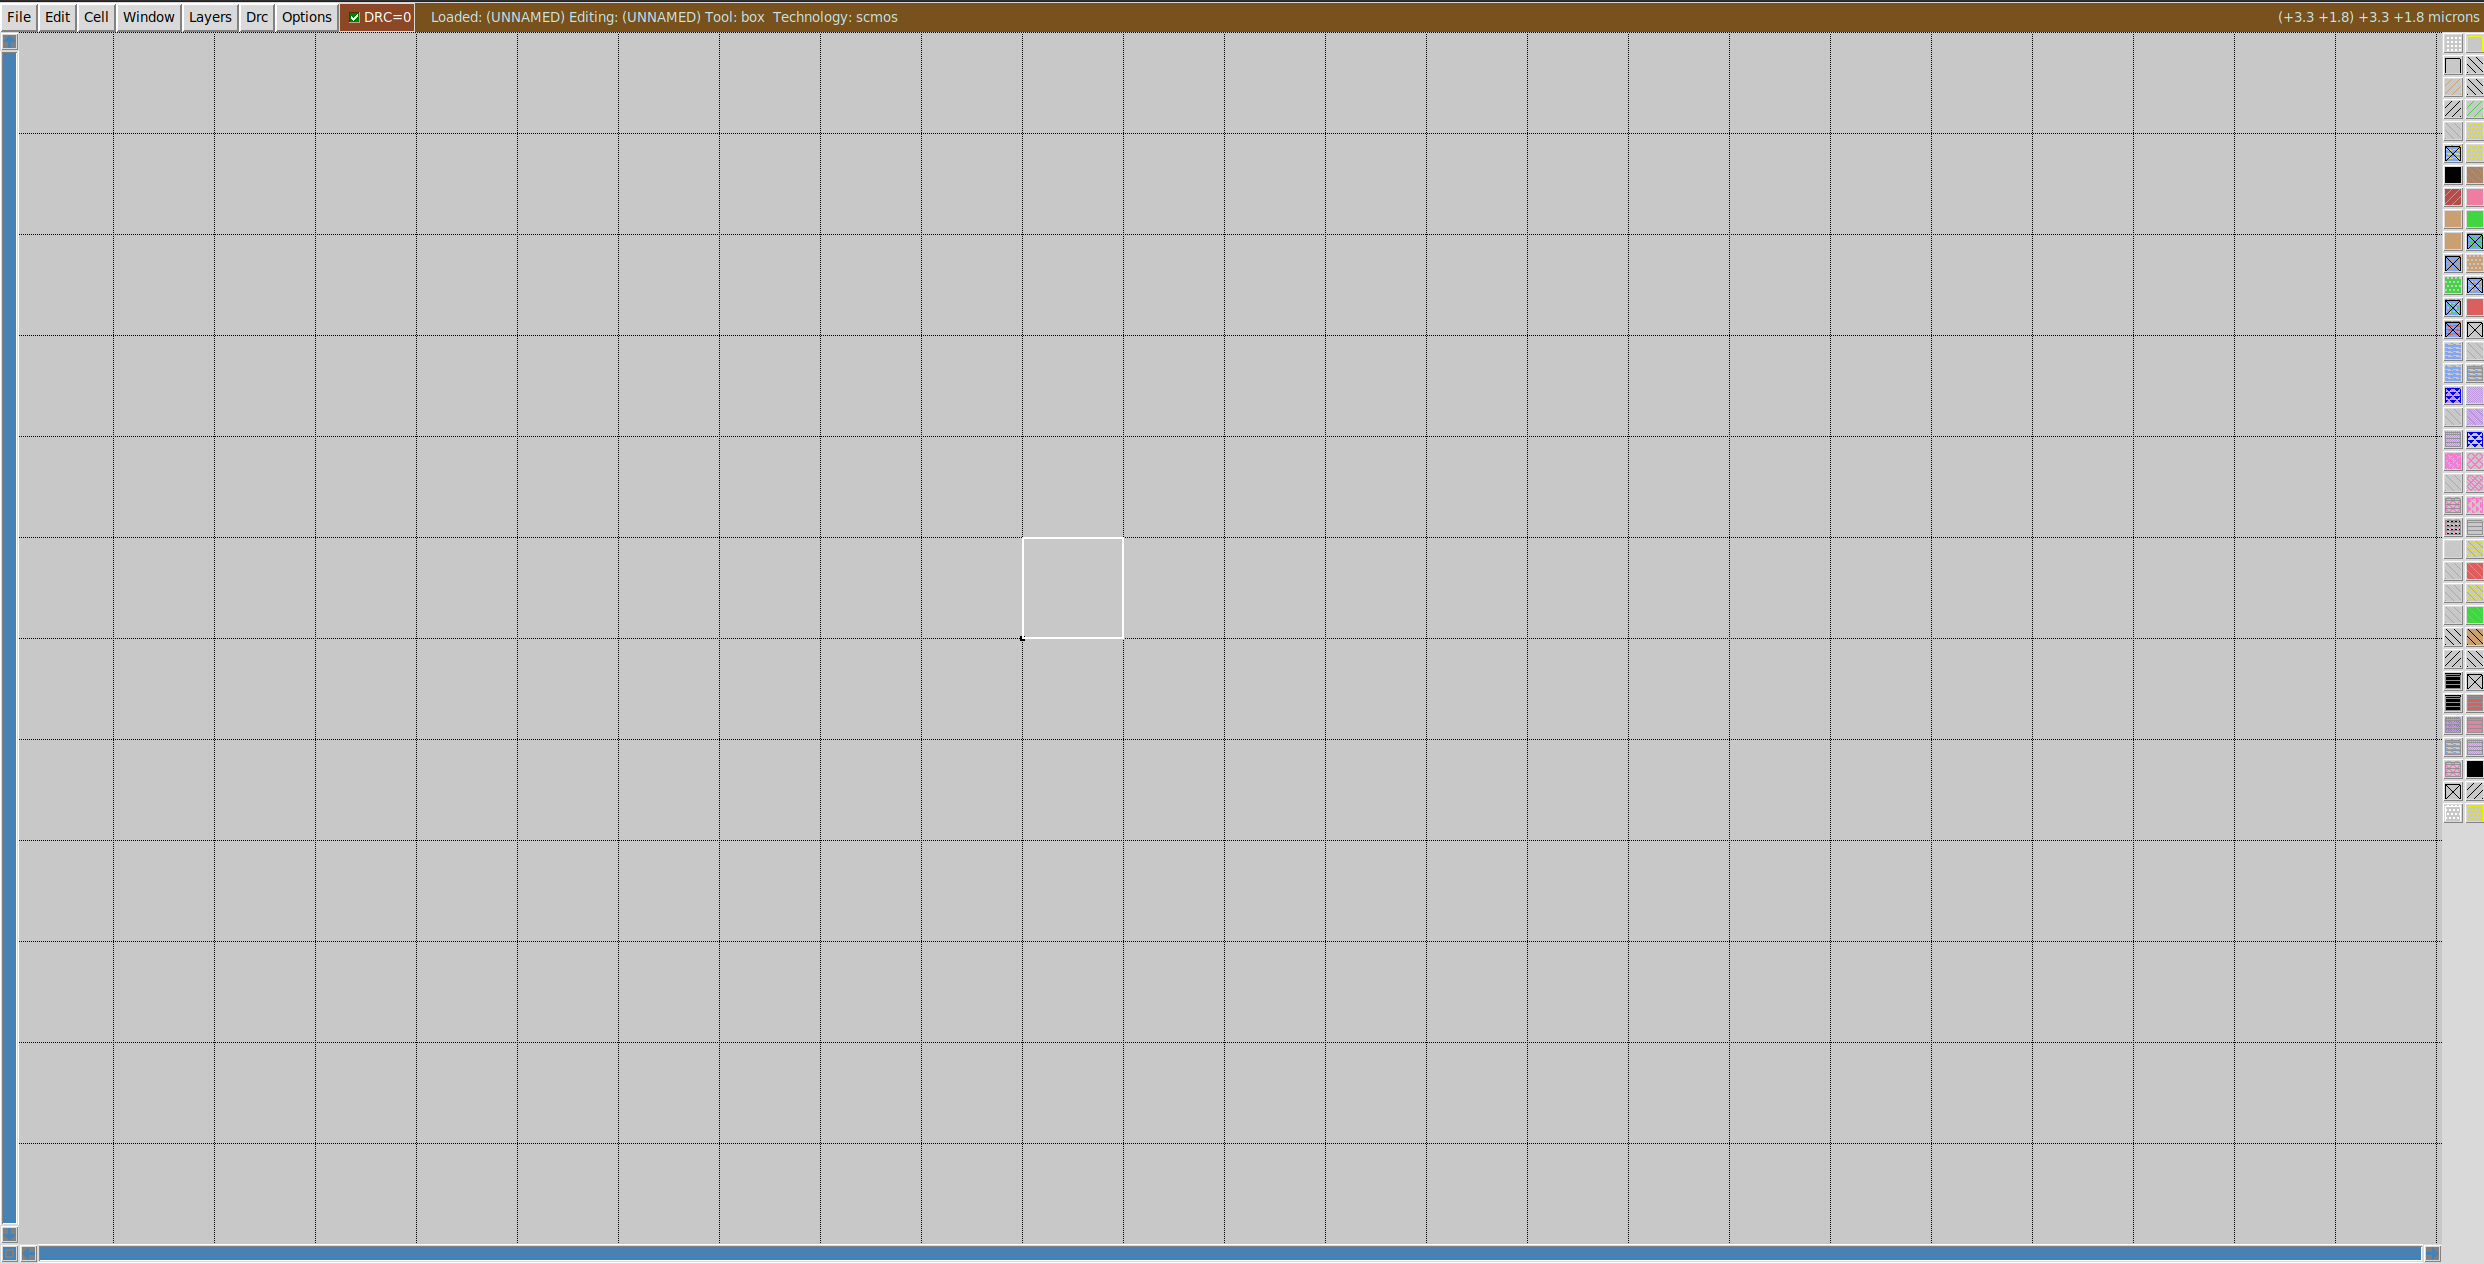
\includegraphics[width=\textwidth]{chapters/chapter2/img/magic_okno}
    \caption{Widok okna programu Magic VLSI.}
    \label{fig:magic_okno}
\end{figure}

\indent Magic VLSI posiada prosty interfejs graficzny,
który składa się z obszaru roboczego, paska narzędzi oraz paska wyboru materiałów.
Dodatkowo wraz z głównym oknem programu otwiera się okno konsoli pozwalające na wprowadzanie dodatkowych komend.
Rysowanie zaczyna się od zaznaczenia obszaru, lewy przycisk myszy służy do wyboru pozycji obszaru,
a prawy do jego rozszerzania.
Aby wypełnić obszar, należy wybrać odpowiedni materiał z paska wyboru
lub z już narysowanych komórek,
poprzez kliknięcie środkowym przyciskiem myszy.
%z tego powodu obecnie można go włączyć jedynie na systemach operacyjnych z rodziny Unix.


\section{Electric}
\section{Microwind}

Microwind to zintegrowane oprogramowanie należące do rodziny EDA (ang. \textit{Electronic Design Automation}),
służące do automatyzacji procesu projektowania układów scalonych lub płytek drukowanych,
umożliwiające projektowanie, symulacje, weryfikacje oraz testowanie układów elektronicznych~\cite{eda}.
Program ten został opracowany przez dra Sicarda do celów edukacyjnych, składa się z kilku modułów,
odpowiadających za różne etapy projektowania układów scalonych~\cite{Microwind}.
Instalacja w przypadku Microwinda jest prosta, wymaga jedynie pobrania pliku instalacyjnego z oficjalnej strony,
a następnie zainstalowania go na komputerze z systemem Windows~\cite{Microwind},
są to natomiast wersje lite (wersja z ograniczoną funkcjonalnością), pełna wersja wymaga licencji.
Dostępna jest także archiwalna pełna wersja programu, która jest dostępna za darmo~\cite{old_microwind}.
Strona zawiera również dokumentację oraz przykłady projektów,
które można wykorzystać w celach edukacyjnych~\cite{Microwind}.\\
\indent Jednym z modułów programu Microwind jest edytor schematów \textbf{Nano Lambda},
pojawiający się domyślnie po uruchomieniu programu.
Posiada dość nieskomplikowany interfejs graficzny z paskiem menu i narzędzi
oraz pływającym oknem palety warstw, przedstawiony na rys.~\ref{fig:microwind_okno}.

\begin{figure}[h]
    \centering
    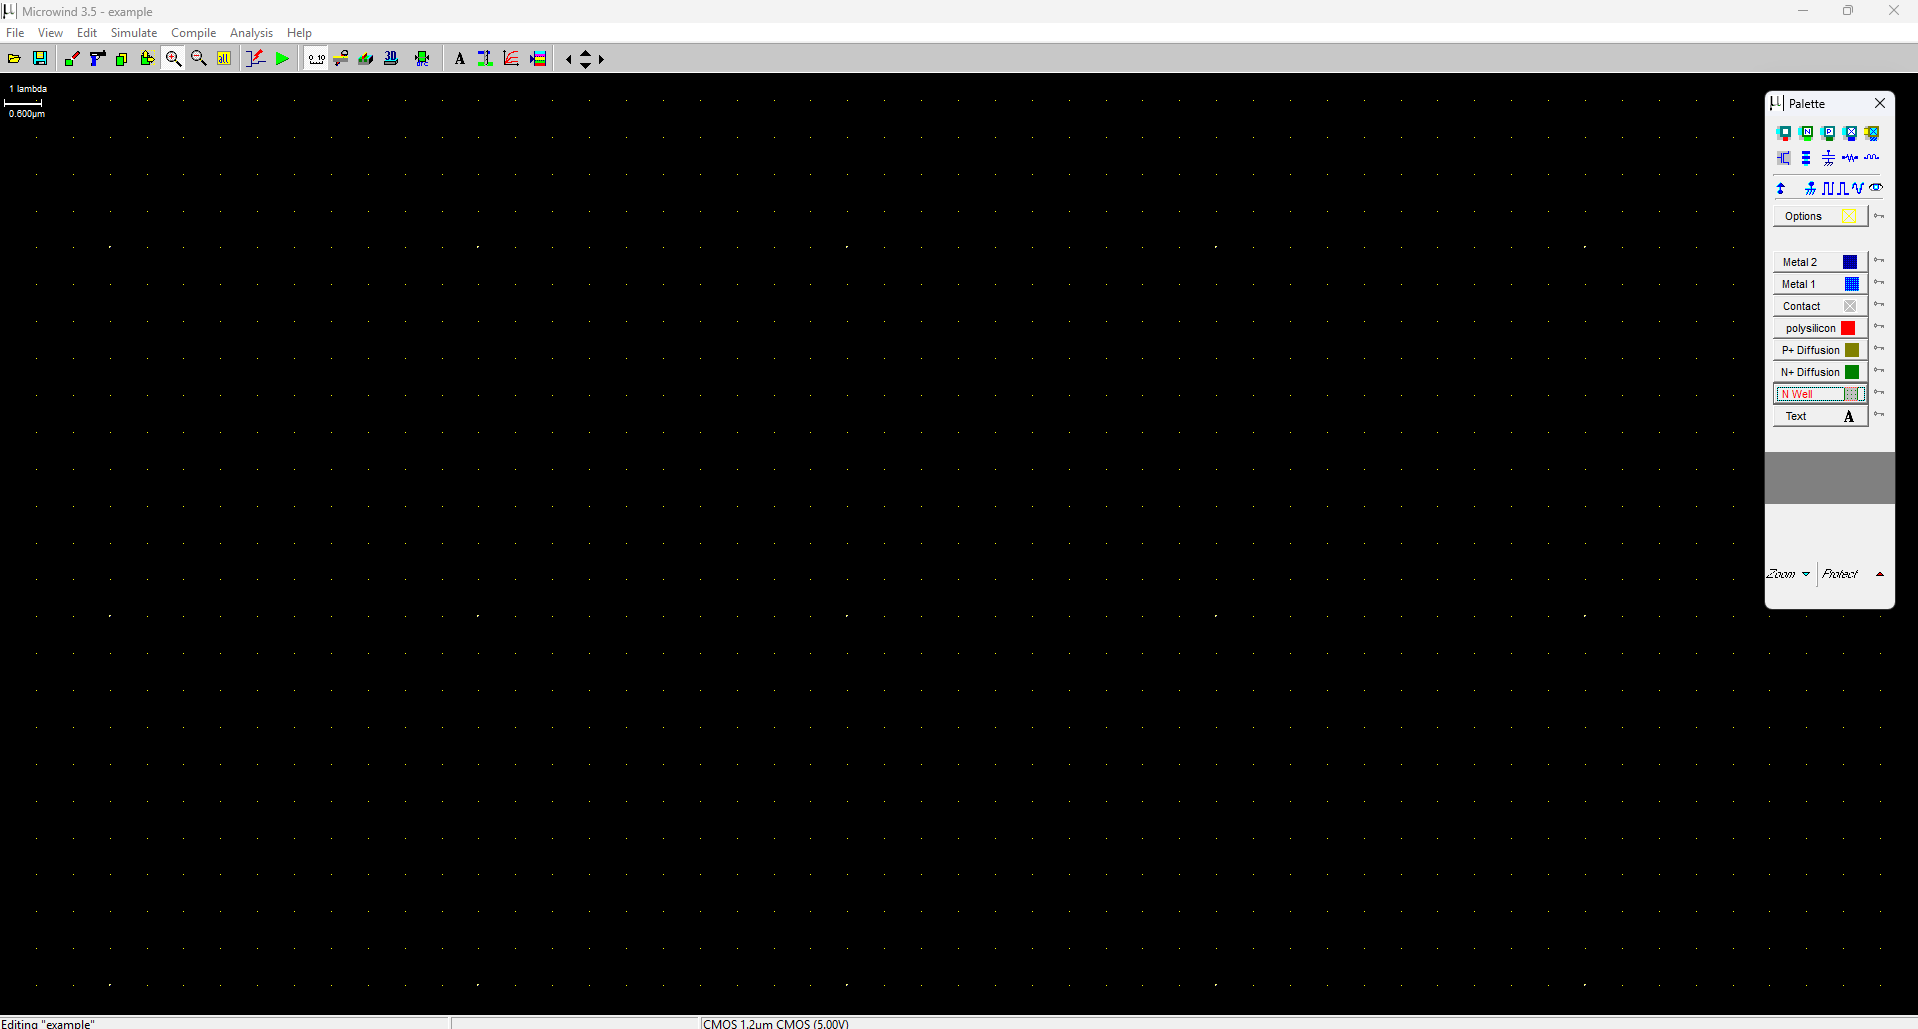
\includegraphics[width=.9\textwidth]{chapters/chapter2/img/microwind_okno}
    \caption[Widok głównego okna programu Microwind.]{Widok głównego okna programu Microwind, źródło:~\cite{Microwind}.}
    \label{fig:microwind_okno}
\end{figure}

\indent Rysowanie odbywa się podobnie jak w przypadku klasycznych edytorów graficznych,
poprzez wybór warstwy z palety,
a następnie przeciągając kursorem po obszarze roboczym przy wciśniętym lewym lub środkowym przycisku myszy,
rysując przy tym prostokątną komórkę.
Nieznaczną wadą rysowania w Microwindzie jest brak przyciągania do siatki,
przez co jest mało precyzyjne.
Przemieszczanie się na obszarze roboczym wymaga używania klawiszy kierunkowych lub przycisków na pasku narzędzi,
co obecnie jest już rozwiązaniem nieergonomicznym.
Program Microwind, poza typowymi narzędziami edycji, charakteryzuje się wieloma zautomatyzowanymi narzędziami,
pozwalającymi generowanie elementów schematów,
na przykład na podstawie funkcji logicznych lub kodu Verilog~\cite{microwind_operation_commands}.\\
\indent Ze względu na brak otwartego kodu źródłowego trudno określić dokładnie zastosowane mechanizmy edytora,
natomiast na podstawie obserwacji można stwierdzić,
że każda edycja schematu wywołuje ponowne rysowanie całego obszaru roboczego,
co jest szczególnie zauważalne podczas usuwania komórek.
Ta sama operacja również wskazuje na strukturę danych, która zakotwiczeniu komórek w kolumnach,
ponieważ po usunięciu obszaru wewnątrz większej komórki, cała kolumna zostaje usunięta.\\
% TODO: poniższe poprawić
\indent Szata graficzna samego edytora charakteryzuje się wysokim kontrastem,
gdzie warstwy są jednolitymi kolorami, częściowo przezroczystymi,
co jest zauważalne, gdy warstwy te się nakładają, przykład przedstawiono na rys.~\ref{fig:microwind_tran}.

\begin{figure}[h]
    \centering
    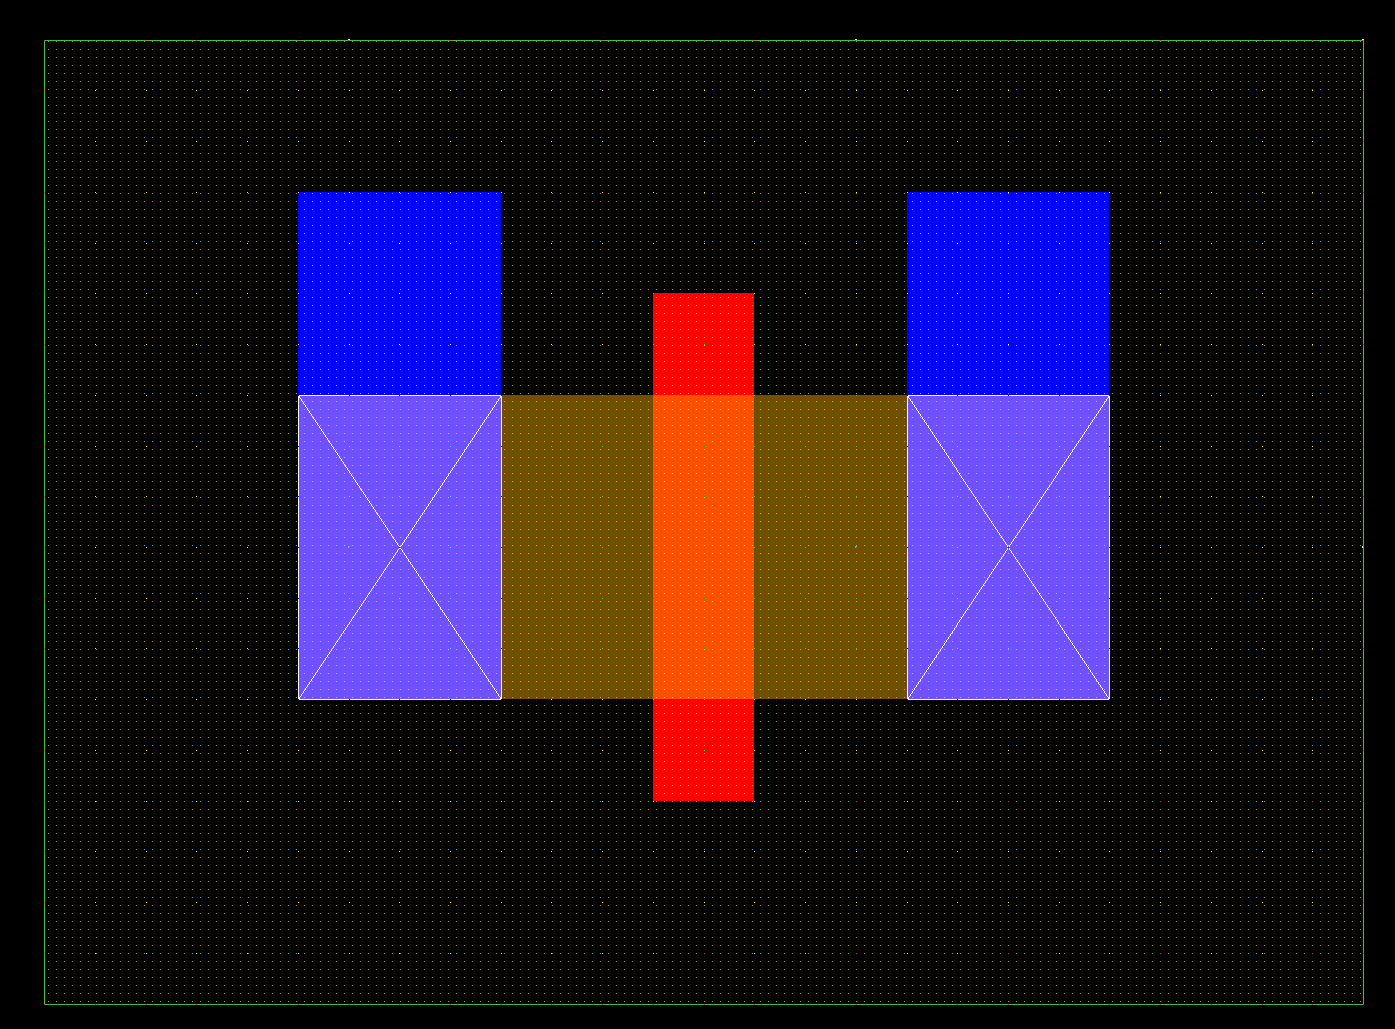
\includegraphics[width=.9\textwidth]{chapters/chapter2/img/microwind_tran}
    \caption[Przykład tranzystora narysowanego w programie Microwind.]
    {
        Przykład tranzystora narysowanego w programie Microwind,
        warstwy \textit{Metal 1}, \textit{P+ Diffusion} oraz \textit{Polysilicon} są jednoilitymi kolorami,
        z wyjątkiem warstwy \textit{N Well} którą reprezentuje kropkowany wzór,
        , źródło: opracowanie własne.
    }
    \label{fig:microwind_tran}
\end{figure}


%\LaTeX{} \cite{VLSI} is a set of macros built atop \TeX{} \cite{texbook}.

\bibliography{main}
\bibliographystyle{unsrt}

\end{document}
